\chapter{Results}\label{chap:results}
This chapter will present the results achieved in the project as described in Chapter \ref{chap:method}. These results include comparisons between different models and their hyperparameters but also a look at the different datasets that were used.

\section{The First Iteration Model}
The first iteration of the model was implemented with no hidden layers, as described in section \ref{sec:modelling_the_ann}. It had an LSTM-RNN layer as its input layer with 30 LSTM units. The hyperparameters of this model are found in table \ref{table:first_iter_parameters}. When this model was trained on a dataset downscaled to contain five users overfitting was achieved as shown in figure \ref{fig:first_iter_overfitting}.
\begin{figure}[h!]
\begin{subfigure}{0.5\textwidth}
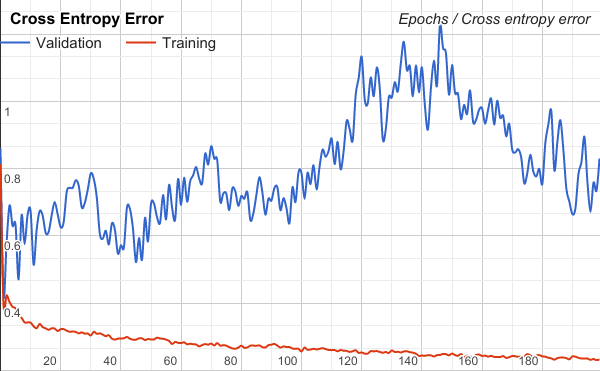
\includegraphics[width=1 \linewidth]{figure/results/first_iter_cross}
\caption{Cross entropy error}
\label{fig:first_iter_overfitting}
\end{subfigure}
\begin{subfigure}{0.5\textwidth}
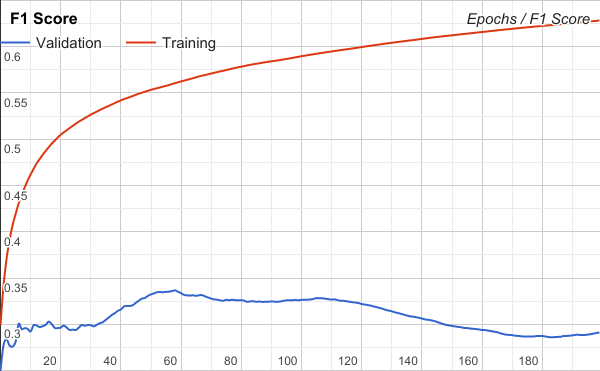
\includegraphics[width=1\linewidth]{figure/results/first_iter_f1}
\caption{$F_1$ score.}
\label{fig:first_iter_f1}
\end{subfigure}
 
\caption{The cross entropy error and $F_1$ score of the first iteration model after 200 training epochs, trained on the training and validation sets. It is good to achieve a low error and a high $F_1$. $F_1$ ranges between $0$ and $1$ inclusive.}
\label{fig:first_iter}
\end{figure}
\\
The best $F_1$ score achieved on the validation set using the model was $0.3366$, as shown in figure \ref{fig:first_iter_f1}. The precision for this model was $0.2554$ and the recall was $0.4936$. As seen in figure \ref{fig:first_iter} the model is overfitting for the training data -- which indicates that the network is learning from the data.
\begin{table}[h!]
    \centering
    \begin{tabular}{ r  l }
        \textbf{Hyperparameter}  &  \textbf{Value} \\ \hline \hline
        Learning rate & $0.5$  \\ \hline
        Vocabulary size & $20000$ \\ \hline
        Batch Size & $25$ \\ \hline
        RNN units & $30$  \\ \hline
        RNN neurons & $200$ \\ \hline
        GRU or LSTM & $LSTM$ \\ \hline
        Embedding Size & $150$ \\ \hline
        Pre-trained embedding matrix & $False$ \\ \hline
        Trainable embedding matrix & $True$ \\ \hline
        Hidden layers & $0$ \\ \hline
        Use $l^2$ regularisation & $False$ \\ \hline
        Use Dropout regularisation & $False$ \\ \hline
        Use constant prediction limit & $False$ \\ \hline
        Use subreddit input & $False$ \\ \hline
        Pre-trained on subreddits & $False$ \\ \hline
    \end{tabular}
    \caption{The hyperparameters for the first iteration model. Non applicable hyperparameters are left out}
    \label{table:first_iter_parameters}
\end{table}

\section{The Final Network}\label{sec:final_model}
After more than 250 different models were tested the most optimal network we managed to achieve for the five user dataset with word stemming had an $F_1$-score of about $0.4548$, as shown in Figure \ref{fig:final_f1}. Figure \ref{fig:final_overfitting} shows that the model started overfitting to the training set after $4047$ epochs. The precision was $0.3552$ and the recall was $0.6368$. The hyperparameters for this final model are shown in table \ref{table:hyperparameters_final}.
\begin{figure}[h!]
\begin{subfigure}{0.5\textwidth}
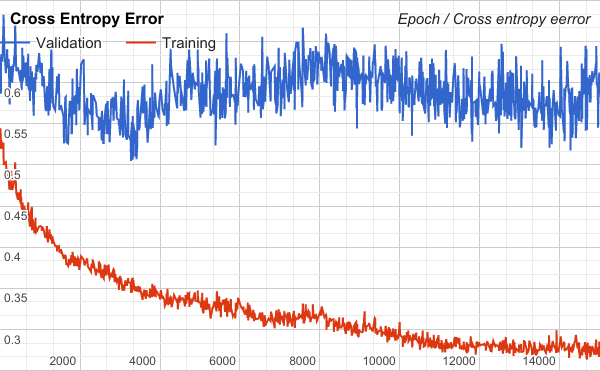
\includegraphics[width=1 \linewidth]{figure/results/stemmed_cross}
\caption{Cross entropy error}
\label{fig:final_overfitting}
\end{subfigure}
\begin{subfigure}{0.5\textwidth}
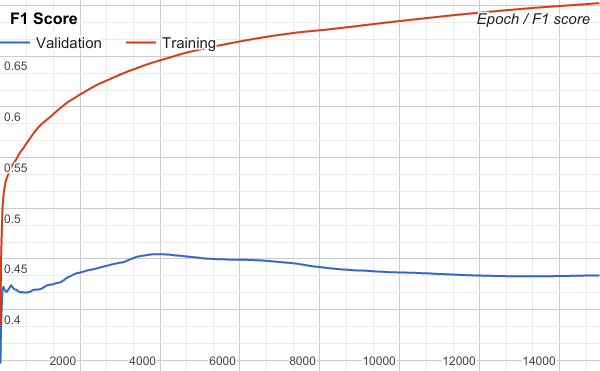
\includegraphics[width=1\linewidth]{figure/results/stemmed_f1}
\caption{$F_1$ score.}
\label{fig:final_f1}
\end{subfigure}
 
\caption{The cross entropy error and $F_1$ score of the final model after 15000 training epochs. It is good to achieve a low error and a high $F_1$. $F_1$ ranges between $0$ and $1$ inclusive.}
\label{fig:final_stemmed}
\end{figure}
\\\\
When the model was upscaled and trained on the dataset with 50 users an $F_1$-score of $0.04802$ was achieved. The precision and recall are shown in table \ref{table:final_all_results}.
\\\\
As the results from the upscaled model did not scale well an attempt on the full non-scaled dataset was never done. The model was used for the word-stemmed dataset, the results for this together with the results for the regular downscaled dataset are shown in table \ref{table:final_all_results}. The model was trained using an Nvidia GTX 1070 graphics card.
\begin{table}[h!]
    \centering
    \begin{tabular}{ r  l }
        \textbf{Hyperparamter}  &  \textbf{Value} \\ \hline \hline
        Learning rate & $0.05$  \\ \hline
        Vocabulary size & $25000$ \\ \hline
        Batch Size & $25$ \\ \hline
        RNN units & $12$  \\ \hline
        RNN neurons & $400$ \\ \hline
        GRU or LSTM & $LSTM$ \\ \hline
        Embedding Size & $300$ \\ \hline
        Pre-trained embedding matrix & $False$ \\ \hline
        Trainable embedding matrix & $True$ \\ \hline
        Hidden layers & $1$ \\ \hline
        Neurons in hidden layers & $300$ \\ \hline
        Use $l^2$ regularisation & $True$ \\ \hline
        $l^2$ Factor & $0.01$ \\ \hline
        Dropout regularisation & $True$\\ \hline
        Dropout probability & $0.75$ \\ \hline
        Use constant prediction limit & $False$ \\ \hline
        Use subreddit input & $False$ \\ \hline
        Pre-trained on subreddits & $False$ \\ \hline
    \end{tabular}
    \caption{The hyperparameters for the final network. Non applicable hyperparameters are left out}
    \label{table:hyperparameters_final}
\end{table}
\\\\
\begin{table}[h!]
    \centering
    \begin{tabular}{ r | c | c }
    & \textbf{5 users dataset} & \textbf{50 users dataset} \\ \hline    \hline
    & \multicolumn{2}{c}{\textbf{Without stemmed dataset}} \\ \hline \hline
    $F_1$-score & $0.3908$ & $0.0480$ \\ \hline
    Precision & $0.2752$ & $0.0249$ \\ \hline
    Recall & $0.6740$ & $0.6538$ \\ \hline \hline
    & \multicolumn{2}{c}{\textbf{With stemmed dataset}} \\ \hline \hline
    $F_1$-score & $0.4548$ & $0.0400$ \\ \hline
    Precision & $0.3552$ & $0.0208$ \\ \hline
    Recall & $0.6318$ & $0.5140$ \\ \hline
    \end{tabular}
    \caption{The $F_1$-score, precision and recall for the final model. The results for both the regular dataset as well as the word-stemmed dataset are shown.}
    \label{table:final_all_results}
\end{table}

\section{Baseline Comparison} 
\label{sec:baseline_comp}
This section presents the results from the different baselines tested. These results will be used when comparing against the artificial neural network model described in section \ref{sec:final_model}. Discussion about the results are left for chapter \ref{chap:discussion}.

\subsection{Facebook fastText Classifier}

The Facebook fastText classifier was tested on the downscaled datasets for 5 and 50 users and with the corresponding pre-processed datasets. The results are shown in table \ref{table:facebook_results}.
\begin{table}[h!]
    \centering
    \begin{tabular}{ r | c | c }
    & \textbf{5 users dataset} & \textbf{50 users dataset} \\ \hline    \hline
    & \multicolumn{2}{c}{\textbf{Without stemmed dataset}} \\ \hline \hline
    $F_1$-score & $0.413$ & $0.118$ \\ \hline
    Precision & $0.413$ & $0.118$ \\ \hline
    Recall & $0.413$ & $0.118$ \\ \hline \hline
    & \multicolumn{2}{c}{\textbf{With stemmed dataset}} \\ \hline \hline
    $F_1$-score & $0.486$ & $0.118$ \\ \hline
    Precision & $0.486$ & $0.118$ \\ \hline
    Recall & $0.486$ & $0.118$ \\ \hline
    \end{tabular}
    \caption{The $F_1$-score, precision and recall for the Facebook fastText classifier. The results for both the regular dataset as well as the word-stemmed dataset are shown.}
    \label{table:facebook_results}
\end{table}

The arguments given to achieve these results can be seen in Table \ref{table:fasttext-arg}

\begin{table}[h!]
    \centering
    \begin{tabular}{ c | c }
    \textbf{Argument} & \textbf{Value} \hline
    -lr & $0.1$ \hline
    -lrUpdateRate & $100$ \hline
    -dim & $10$ \hline
    -ws & $5$ \hline
    -epoch & $1000$ \hline
    -minCount & $1$ \hline
    -minCount & $0$ \hline
    -neg & $5$ \hline
    -wordNgram & $2$ \hline
    -loss & ns \hline
    -bucket & $10 000 000$ \hline
    -minn & $0$ \hline
    -maxn & $0$ \hline
    -thread & $8$ \hline
    -t & $0.00001$ \hline
    --pretrainedVectors & []
    \end{tabular}
    \caption{Arguments used to get the recorded results for fastText}
    \label{table:fasttext-arg}
\end{table}

\subsection{N-grams}
The N-grams based model was tested on the downscaled dataset with five users and with the corresponding pre-processed dataset. The results are shown in table \ref{table:ngram_results}.
\begin{table}[h!]
    \centering
    \begin{tabular}{ r | c | c }
     & \textbf{5 users dataset} & \textbf{50 users dataset} \\ \hline \hline
     & \multicolumn{2}{c}{\textbf{Without stemmed dataset}} \\ \hline \hline
    $F_1$-score & $0.3898$ & -- \\ \hline
    Precision & $0.2777$ & -- \\ \hline
    Recall & $0.6536$ & -- \\ \hline \hline
    & \multicolumn{2}{c}{\textbf{With stemmed dataset}} \\ \hline \hline
    $F_1$-score & $0.4044$ & -- \\ \hline
    Precision & $0.2898$ & -- \\ \hline
    Recall & $0.6686$ & -- \\ \hline
    \end{tabular}
    \caption{The $F_1$-score, precision and recall for the N-grams based model. The results for both the regular dataset as well as the word-stemmed dataset are shown.}
    \label{table:ngram_results}
\end{table}
\\\\
Due to computational complexity a result for the dataset with 50 users could not be achieved for this baseline.

\section{Analysis of the Datasets}
\label{sec:dataset-summary}
This section presents the result of the investigation into the different datasets used. The goal of this was to see if there were any irregularities or patterns in the datasets that could have had an affect on the performance of the networks or the baselines.

\subsection{Downscaled Dataset with 5 Users}
\label{sec:five-user-data-set}
It was found in the training set for the downscaled five user dataset that the difference in length of the longest title and the second longest title was large. The longest title was $1928$ words while the second longest was $66$ words. This skewed the variance for the training data and is why the standard deviation is $24.9$, as seen in table \ \ref{table:5_user_stats}. If the outlier is removed, the standard deviation is brought down to $9.7$ which is similar to the validation and testing sets.
\begin{table}[H]
    \centering
    \begin{tabular}{ r | c | c | c }
    \textbf{Feature} & \textbf{Training} & \textbf{Validation} & \textbf{Testing} \\ \hline \hline
    \multicolumn{4}{c}{\textbf{Titles}} \\ \hline \hline
    Amount & 6927 & 1983 & 992 \\ \hline
    Median length & 9 & 9 & 8 \\ \hline
    Average length & 12 & 11 & 11  \\ \hline
    Title length $\sigma$ & 24.9 & 9.6 & 9.4 \\ \hline
    Longer than average & 2198 & 696 & 320 \\ \hline
    More than 1 vote & 76 & 9 & 6 \\ \hline
    More than 2 votes & 2 & 0 & 0\\ \hline \hline
    \multicolumn{4}{c}{\textbf{Subreddits}} \\ \hline \hline
    Amount & 103 & 65 & 59  \\ \hline
    Average voted in in & 32.2 & 21.8 & 19.4 \\ \hline
    Voted in $\sigma$ & 18.4 & 11.49 & 10.2  \\ \hline
    \end{tabular}
    \caption{Statistics regarding title length, votes and subreddits for the downscaled dataset containing five users}
    \label{table:5_user_stats}
\end{table}
The analysis also showed that few users shared liked titles. In the training set only about $1\%$ of titles have more than $1$ vote -- in the validation and testing sets that number is even less, as shown in table \ref{table:5_user_stats}.
\begin{table}[H]
    \centering
    \begin{tabular}{ r | c | c | p{4cm}  }
    \textbf{User} & \textbf{Subreddits} & \textbf{Total votes} & \textbf{Votes in two most voted subreddits} \\ \hline \hline
    \multicolumn{4}{c}{\textbf{Training data set}} \\ \hline \hline
    Ayavaron & 64 & 1411 & 444 \\ \hline
    akkartik & 14  & 1387 & 1333 \\ \hline
    crmaki & 14 & 1410 & 902 \\ \hline
    izzycat & 37 & 1363 & 505 \\ \hline
    doctorgonzo & 32 & 1429 & 586 \\ \hline \hline
    \multicolumn{4}{c}{\textbf{Validation data set}} \\ \hline \hline
    Ayavaron & 40 & 416 & 133 \\ \hline
    akkartik & 8  & 392 & 372 \\ \hline
    crmaki & 11 & 390 & 252 \\ \hline
    izzycat & 26 & 428 & 158 \\ \hline
    doctorgonzo & 24 & 364 & 146 \\ \hline \hline
    \multicolumn{4}{c}{\textbf{Testing data set}} \\ \hline \hline
    Ayavaron & 33 & 172 & 60 \\ \hline
    akkartik & 5  & 220 & 212 \\ \hline
    crmaki & 12 & 194 & 131 \\ \hline
    izzycat & 19 & 207 & 77 \\ \hline
    doctorgonzo & 28 & 204 & 78 \\ \hline
    \end{tabular}
    \caption{Vote distribution showing votes in subreddits, total votes and votes in the top two voted subreddits for each user in the training, validation and testing data sets with five users}
    \label{table:5_user_density}
\end{table}
The vote density for the downscaled five user dataset is shown in table \ref{table:5_user_density}. The table shows statistics for the training, validation and testing sets. It summarises how many subreddits a user has voted in, the total number of votes a user has and how many votes a user has made in the two subreddits that the user has voted most in.

\subsection{Downscaled Dataset with 50 Users}
Compared to the downscaled dataset with five users there are no big outliers in the downscaled dataset with $50$ users. There are however a higher percentage of users that share liked titles in comparison. As seen in table \ref{table:50_user_stats}, for the training set, $7.75\%$ of titles have more than one vote. In the validation set it is $6\%$ and for the testing set it is $5.7\%$.
\\\\
\begin{table}[H]
    \centering
    \begin{tabular}{ r | c | c | c }
    \textbf{Feature} & \textbf{Training} & \textbf{Validation} & \textbf{Testing} \\ \hline \hline
    \multicolumn{4}{c}{\textbf{Titles}} \\ \hline \hline
    Amount & 63176 & 18486 & 9301 \\ \hline
    Median length & 9 & 9 & 9 \\ \hline
    Average length & 12 & 12 & 12  \\ \hline
    Title length $\sigma$ & 11.7 & 9.3 & 9.3 \\ \hline
    Longer than average & 23474 & 6736 & 3354 \\ \hline
    More than 1 vote & 5428 & 1231 & 577 \\ \hline
    More than 2 votes & 980 & 220 & 92\\ \hline \hline
    \multicolumn{4}{c}{\textbf{Subreddits}} \\ \hline \hline
    Amount & 343 & 248 & 192  \\ \hline
    Average voted in in & 31.28 & 22.6 & 18.58 \\ \hline
    Voted in $\sigma$ & 17.6 & 12.17 & 9.88  \\ \hline
    \end{tabular}
    \caption{Statistics regarding title length, votes and subreddits for the downscaled dataset containing 50 users}
    \label{table:50_user_stats}
\end{table}
The statistics regarding the vote density, similar to the one in table \ref{table:5_user_density}, for the $50$ users datasets have been left out simply due to the space of the table it would require. However, most of the Reddit posts in the 50 user dataset have a low number of votes.
